%%%%%%%%%%%%%%%%%%%%%%%%%%%%%%%%%%%%%%%%%%%%%%%%%%%%%%%%%%%%%%%%%%%%%%%%%%%%%%%
%% DDKWizard documentation
%%
%% $Id: DDKWizard_Help.tex 29 2008-06-27 00:11:35Z oliver $
%%%%%%%%%%%%%%%%%%%%%%%%%%%%%%%%%%%%%%%%%%%%%%%%%%%%%%%%%%%%%%%%%%%%%%%%%%%%%%%
\documentclass[a4paper,titlepage]{report}
\usepackage{ae}
\usepackage[T1]{fontenc}
\usepackage[ansinew]{inputenc}
\usepackage[english]{babel}
\usepackage[english]{varioref}
\usepackage{color}
\usepackage{fancybox}
\usepackage{float}
\usepackage[
    colorlinks=true,
    linkcolor=black,
    citecolor=black,
    urlcolor=black,
    menucolor=black,
    filecolor=black,
    breaklinks=false,
    bookmarksnumbered=false,
    pdfstartview=FitH,
    pdftitle={DDKWizard Manual},
    pdfkeywords={DDKBUILD, DDKWizard, Oliver Schneider, Assarbad, DDK, Visual Studio, Project Templates, Wizard, DDK project, DDK project wizard, DDK wizard, WDK, Driver Development Kit, Windows Driver Kit},
    pdfsubject={Manual for DDKBUILD and DDKWizard with its project templates},
    pdfcreator={LaTeX},
    pdfauthor={Oliver Schneider (assarbad.net)}
    ]{hyperref}
%\usepackage{lscape} %landcape pages support
\usepackage{fancyhdr}
\usepackage{fancyvrb}
\usepackage{datetime}
\usepackage[pdftex]{graphicx}

\addtolength{\textwidth}{3cm}
\addtolength{\textheight}{0.7cm}
\setlength{\oddsidemargin}{0cm}
\setlength{\evensidemargin}{0cm}
\setlength{\headheight}{0mm}
\setlength{\topmargin}{0mm}

\definecolor{gray}{gray}{0.5}
\newcommand{\marginlabel}[1]{\mbox{}\marginpar{\raggedright\hspace{0pt}\footnotesize{\textsf{#1}}}}
\newcommand{\linkclr}[1]{\textcolor[rgb]{0.00,0.00,0.60}{#1}}
\newcommand{\important}[1]{\textcolor[rgb]{0.90,0.00,0.00}{\textbf{#1}}}
\newcommand{\msdn}[1]{\href{http://search.msdn.microsoft.com/search/default.aspx?siteId=0&tab=0&query=#1}{\texttt{\linkclr{#1}()}}}
\newcommand{\extlink}[2]{\href{#1}{\linkclr{#2}}}
\newcommand{\extlinktt}[2]{\href{#1}{\texttt{\linkclr{#2}}}}
\newcommand{\googleex}[2]{\href{http://www.google.com/search?q=#1&num=25&ie=utf-8&oe=utf-8}{\linkclr{#2}}}
\newcommand{\google}[1]{\googleex{#1}{#1}}
\newcommand{\default}[1]{\textcolor[gray]{0.40}{(default: \texttt{#1})}}
\newcommand{\option}[1]{\textcolor[rgb]{0.00,0.20,0.20}{\textsf{#1}}}
\newcommand{\optiondeco}[1]{#1\vspace{0.1cm}}
\newcommand{\inioption}[1]{\\\textcolor[rgb]{0.00,0.00,0.40}{\textsl{Value name:} \texttt{#1}}}
\def\ddkwiz{D\kern-.09em D\kern-.09em K\kern-.20em \raise-.20ex\hbox{W}\kern-.15em\raise.20ex\hbox{\it{i}}\kern-.02em{zard}}
\newcommand{\ddkwizver}[0]{\ddkwiz{} v1.2.0a}
\newcommand{\prefast}[0]{\textsf{PRE\textsl{f}ast}}
\newcommand{\solcfg}[2]{\texttt{#1 free} and \texttt{#1 checked}:\\#2}
\newcommand{\solcfgsixfour}[2]{\texttt{#1 free} and \texttt{#1 checked} \textcolor[gray]{0.40}{\textsf{\small(only if 64bit support was activated)}}:\\#2}
\newcounter{copyrightyear}
\setcounter{copyrightyear}{\the\year}
% Date format
\newdateformat{isodate}{\THEYEAR-\twodigit{\THEMONTH}-\twodigit{\THEDAY}}

\setlength{\parindent}{0mm}
\renewcommand{\headrule}{{\color{gray}\hrule height\headrulewidth width\headwidth}}

% Heading styles
\pagestyle{fancy}
%\renewcommand{\chaptermark}[1]{\markboth{\chaptername \ \thechapter.\ #1}{}}
\renewcommand{\chaptermark}[1]{\markboth{#1}{}}
\renewcommand{\sectionmark}[1]{}
\renewcommand{\subsectionmark}[1]{}
\newcommand{\myleftfooter}[0]{\footnotesize{\textsf{\href{http://ddkwizard.assarbad.net}{\textcolor[gray]{0.5}{\copyright~2006-\arabic{copyrightyear} Oliver Schneider}}}}}
\newcommand{\myrightfooter}[0]{\footnotesize{\textsf{\textcolor[gray]{0.5}{$ $Revision: 29 $ $}}}}
\newcommand{\myleftheader}[0]{\textsf{\textcolor[gray]{0.5}{\ddkwizver{} Manual}}}
\newcommand{\myrightheader}[0]{\textsf{\textcolor[gray]{0.5}{\leftmark}}}
\lfoot[\fancyplain{\myleftfooter}{\myleftfooter}]{\fancyplain{\myleftfooter}{\myleftfooter}}
\cfoot[\fancyplain{\textsf{\thepage}}{\textsf{\thepage}}]{\fancyplain{\textsf{\thepage}}{\textsf{\thepage}}}
\rfoot[\fancyplain{\myrightfooter}{\myrightfooter}]{\fancyplain{\myrightfooter}{\myrightfooter}}
\lhead[\fancyplain{\myleftheader}{\myleftheader}]{\fancyplain{\myleftheader}{\myleftheader}}
\rhead[\fancyplain{\myrightheader}{\myrightheader}]{\fancyplain{\myrightheader}{\myrightheader}}
%Published under the ... license
\fontfamily{cmss}
\begin{document}
%%%%%%%%%%%%%%%%%%%%%%%%%%%%%%%%%%%%%%%%%%%%%%%%%%%%%%%%%%%%%%%%%%%%%%%%%%%%%%%
%% Title page
%%%%%%%%%%%%%%%%%%%%%%%%%%%%%%%%%%%%%%%%%%%%%%%%%%%%%%%%%%%%%%%%%%%%%%%%%%%%%%%
\pdfbookmark[0]{Front page}{Titlepage}
\begin{titlepage}
\begin{center}
\large \ddkwizver{} Manual\\
\vskip 2cm
\textbf{\huge{How to use \ddkwiz{}}}
\vskip 2cm
\begin{itemize}
\item{\large{Setup of \texttt{DDKBUILD}}}
\item{\large{Usage of the wizard}}
\item{\large{Configuration of the wizard}}
\item{\large{Tech-speak ...}}
\item{\large{Frequently Asked Questions (FAQ)}}
\item{\large{Deutsche Informationen}}
\end{itemize}
\vskip 2.5cm
\textsf{{\emph{\textcolor[gray]{0.75}{May the source be with you, stranger ... ;-)}}}\\}
\vskip 3.25cm
\textsc{Created:} \isodate\today\\
\textsc{Author:} \href{http://assarbad.net/en/contact}{Oliver Schneider}\\
\vskip 0.7cm
Copyright \copyright\hspace{0.1ex}~2006-\arabic{copyrightyear} Oliver Schneider (\textsf{\href{http://assarbad.net}{\linkclr{assarbad.net}}})
{\small\color{gray}\verb+$Id: DDKWizard_Help.tex 29 2008-06-27 00:11:35Z oliver $+}\\

\addvspace{0.5cm}
{\small\color{gray}\textsf{Trademarks appear throughout this text
without any trademark symbol; they are the property of their respective
trademark owner. There is no intention of infringement; the usage is to
the benefit of the trademark owner.}}
\end{center}
\end{titlepage}
%%%%%%%%%%%%%%%%%%%%%%%%%%%%%%%%%%%%%%%%%%%%%%%%%%%%%%%%%%%%%%%%%%%%%%%%%%%%%%%
%% /Title page
%%%%%%%%%%%%%%%%%%%%%%%%%%%%%%%%%%%%%%%%%%%%%%%%%%%%%%%%%%%%%%%%%%%%%%%%%%%%%%%
\chapter*{Preface\markboth{Preface}{}}\thispagestyle{fancy}
\ddkwiz{} was written \textbf{because I can be very lazy}, plain and simple!\\

It is a laziness that is so irrational if you think about it twice.
Programmers tend to spend hours to solve a problem \emph{generically}\texttrademark{}
instead of solving it specifically and tailored to the specific problem within a few
minutes (but potentially over and over again).\\

When I started using OSRs \texttt{DDKBUILD.BAT} script\footnote{Which was a traditional batch script.}
I soon thought I could rewrite it to make use of all these neat tricks
that are allowed by the NT script interpreter\footnote{The NT script interpreter
goes indeed far beyond what batch provides!}. You can just download the original
version (\texttt{.bat}) as well as the rewritten one (\texttt{.cmd}) from
\extlink{http://www.osronline.com/article.cfm?article=43}{OSR Online}\footnote{You need to be logged on to download the files.}
or from the \ddkwiz{} website at \extlinktt{http://ddkwizard.assarbad.net}{ddkwizard.assarbad.net}.
Soon, however, the need for generic \texttt{DDKBUILD} project creation became ``overwhelming'' ...\\

As a side-note: There is another\footnote{... as far as I know the continuation of
the very first \texttt{DDKBUILD} script.} \texttt{DDKBUILD} script from Mark Roddy at
\extlinktt{http://www.hollistech.com}{www.hollistech.com}
that does the same as the two scripts from OSR. However, I did not take the time
to check the compatibility issues that may arise from usage of \ddkwiz{} together
with this \texttt{DDKBUILD} ``flavor''. If someone ever does it, please let me know
and I will probably modify \ddkwiz{} to incorporate the necessary
settings. Currently it relies on the fact that the batch and the NT script
versions from OSR take the same arguments, so using it with ``the other''
\texttt{DDKBUILD} is not recommended, but of course you can try it if you are curious.

\section*{Compatibility} \ddkwiz{} works with the DDKs of
Windows 2000, Windows XP, Windows 2003 Server and newer WDKs (Windows Driver Kits).
It does not include any configurations for WDF projects and may never include
them in future. I'll just wait for feedback before deciding about it.\\
It is compatible with Visual Studio .NET, Visual Studio .NET 2003, Visual Studio 2005,
Visual Studio 2008 and the express editions of Visual C++ 2005 and 2008. The ``normal''
Visual C++ versions are supposed to work fine as well. Refer to \autoref{sec:propsheets}
and \autoref{compat:activex} for some possible limitations depending
on your Visual Studio version.\\
Visual Studio 2005 and 2008 (and its flavors) support all \ddkwiz{} features!

\section*{Prerequisites}
\begin{description}
  \item[\texttt{DDKBUILD}:] First of all you need to set up your copy of \texttt{DDKBUILD} according to the version
that you downloaded. It may sound strange (and ``selfish''), but I recommend to
use the NT script (\texttt{.cmd}) version since it provides extra functionality
(see \autoref{subsec:buildscripts})
which can be handy sometimes. Setup of the batch version is explained in \autoref{sec:batchversion},
while the NT script version is explained in \autoref{sec:ntscriptversion}.
  \item[Laziness:]
  You need to be extraordinarily lazy\footnote{And for those who didn't get it just yet - yes, this is a joke.}
  to even install this wizard! If you are not lazy enough, that is below 7 on a laziness scale from 1 to 10, you
must not use this wizard.
\textbf{Warning: having this wizard installed on your workstation in your
company will be a clear hint to your boss that you are lazy. So be careful when
installing and using it \textsf{;-)}.}\footnote{Luckily my current employer accepts
this form of laziness in exchange for the increased productivity \textsf{;-)}.}
\end{description}

\section*{How to use this manual}
If you are viewing this document in a PDF viewer, you can take advantage of the
clickable elements such as links to external websites and links between
chapters and sections - click the chapter, section or footnote numbers to
see the referenced item. Also if you visit the \emph{Contents} at the end of
this document you can click the items there (not the page numbers, though).
This should make it easier for you to navigate the document and follow
back and forward references which occur every now and then --- yet it leaves
the document in a state where it can be printed out conveniently.\\
Kindly note that I use the terms WDK and DDK interchangeably. Unless I want to
refer to a specific version, I try to stick to the traditional term DDK.

\section*{Do you like \ddkwiz{}? Donations \& contributions}
If you like \ddkwiz{}, please consider donating to any charity organization you
like and trust. But don't feel forced, I wrote
it primarily to satisfy my own laziness and the laziness of others \textsf{;-)}.\\

Also, you will certainly help a lot by providing feedback about possible bugs,
feature requests and of course praise. \important{Contributions (new templates,
better source files in existing templates) are \emph{very} welcome.}

\section*{Website}
The website of \ddkwiz{} is at \extlinktt{http://ddkwizard.assarbad.net}{ddkwizard.assarbad.net}.
There you will find this documentation for download as well as the latest
version of the templates and their installer.

\section*{An advice}
Nah, of course this is not ``adware''. I'd just like to point out how much
I liked the two seminars with Mark from OSR and send some greetings to
him and the other guys over at OSR. I like the published books, the mailing
lists, \emph{The NT Insider} and their commitment to the NT driver community!
If you have to work with drivers professionally you \emph{have} to take at least
one of their seminars\footnote{... and not be too shy to ask a lot of ``stupid''
questions \textsf{;-)}} - \textbf{you have to!}

%%%%%%%%%%%%%%%%%%%%%%%%%%%%%%%%%%%%%%%%%%%%%%%%%%%%%%%%%%%%%%%%%%%%%%%%%%%%%%%
%% LICENSE TEXT
%%%%%%%%%%%%%%%%%%%%%%%%%%%%%%%%%%%%%%%%%%%%%%%%%%%%%%%%%%%%%%%%%%%%%%%%%%%%%%%
\chapter*{License\markboth{License}{}\pdfbookmark[0]{License}{License}}\thispagestyle{fancy}

The following license applies to all parts of \ddkwiz{}, \emph{except for any actual
project templates}.\\

\begin{verbatim}
Copyright (c) 2006-2008 by Oliver Schneider (assarbad.net)

This software is provided 'as-is', without any express or implied warranty. In
no event will the authors be held liable for any damages arising from the use
of this software.

Permission is granted to anyone to use this software for any purpose, including
commercial applications, and to alter it and redistribute it freely, subject to
the following restrictions:

  1. The origin of this software must not be misrepresented; you must not claim
     that you wrote the original software. If you use this software in a product,
     an acknowledgment in the product documentation would be appreciated but is
     not required.

  2. Altered source versions must be plainly marked as such, and must not be
     misrepresented as being the original software.

  3. This notice may not be removed or altered from any source distribution.
\end{verbatim}

The \emph{included} project templates are all in the \texttt{PUBLIC DOMAIN}, but the same
disclaimer, as stated in the above license, applies:

\begin{verbatim}
This software is provided 'as-is', without any express or implied warranty. In
no event will the authors be held liable for any damages arising from the use
of this software.
\end{verbatim}

Actually the files, once you create a project with \ddkwiz{}, will contain your
copyright if you configure the values for \texttt{Author} and \texttt{CompanyName}
as described in \autoref{sec:authorandcompany} and you have at least Visual
Studio 2005.

%%%%%%%%%%%%%%%%%%%%%%%%%%%%%%%%%%%%%%%%%%%%%%%%%%%%%%%%%%%%%%%%%%%%%%%%%%%%%%%
%% CHAPTER 1
%%%%%%%%%%%%%%%%%%%%%%%%%%%%%%%%%%%%%%%%%%%%%%%%%%%%%%%%%%%%%%%%%%%%%%%%%%%%%%%
\chapter{Setup of \texttt{DDKBUILD}}\thispagestyle{fancy}
\section{\texttt{DDKBUILD.BAT}}
\label{sec:batchversion}
This is the classic. \texttt{DDKBUILD.BAT} is easily installed by following these
few steps:
\begin{enumerate}
  \item
    Download \texttt{DDKBUILD.BAT} from \extlink{http://www.osronline.com/article.cfm?article=43}{this page}
    or \extlinktt{http://ddkwizard.assarbad.net}{ddkwizard.assarbad.net}.
  \item
    Copy \texttt{DDKBUILD.BAT} into a directory where you want it to reside. I usually
    choose a directory that can be accessed from anywhere else. Let us say you have
    the DDKs for Windows XP and 2003 installed and they are located in \verb+C:\WINDDK\2600+
    and \verb+C:\WINDDK\3790.1830+ respectively. Now you could copy \texttt{DDKBUILD.BAT}
    into the common root folder of your DDKs, in our case \verb+C:\WINDDK+.
  \item \label{item:envvar1}
    Append the path to the directory where \texttt{DDKBUILD.BAT} resides to the \texttt{PATH}
    variable of either your user account or to the system-wide \texttt{PATH} variable. In
    either case right-click \emph{My Computer} and choose \emph{Properties}. Then go to the
    \emph{Advanced} page and click \emph{Environment Variables}. There you can add or edit
    the PATH variable of the system\footnote{... if you are an administrator.} or your user
    account. Note that the values for the variable are delimited by semi-colons (``\texttt{;}'').
    \autoref{fig:EnvironmentVariables} shows the dialog. Leave the dialog open for
    \autoref{item:envvar2}.\\
    Leaving out this step will still enable you to use \texttt{DDKBUILD.BAT} from within
    your IDE but will prevent you from using it conveniently from the command line.
  \item
    Start up your Visual Studio\footnote{Referring to Visual Studio I mean specifically
    Visual C++.} IDE and from the \emph{Tools} menu choose \emph{Options} and in the left
    navigation pane choose the folder \emph{Projects and Solutions} and then \emph{VC++ Directories}.
    From the combobox \emph{Show directories for} choose \emph{Executable files} and add the
    path of the directory where \texttt{DDKBUILD.BAT} resides here as well.
    \autoref{fig:VisualStudioToolsDialog} shows the dialog.
  \item \label{item:envvar2}
    Depending on the DDKs you have installed, you should set the variables\footnote{It is your
    choice whether you set the system-wide variables or those for your user account.} (using
    the dialog opened before, in \autoref{item:envvar1}) with the following names to point to the
    respective directories\footnote{For the NT4 DDK you can use the \texttt{NT4BASE} variable.
    However, this is not supported by \ddkwiz{}.}:
    \begin{itemize}
        \item
          \textbf{Windows 2000 DDK:}\\
            For this DDK set the variable \texttt{W2KBASE} to point to the base directory of your
            Windows 2000 DDK.
        \item
          \textbf{Windows XP DDK:}\\
            For this DDK set the variable \texttt{WXPBASE} to point to the base directory of your
            Windows XP DDK. For the example in the first point this would be \verb+C:\WINDDK\2600+.
        \item
          \textbf{Windows 2003 Server DDK:}\\
            For this DDK set the variable \texttt{WNETBASE} to point to the base directory of your
            Windows 2003 Server DDK. For the example in the first point this would be \verb+C:\WINDDK\3790.1830+
            (which would be a typical path to the 2003 SP1 DDK).
        \item
          \textbf{Windows Vista/Windows 2008 Server WDK:}\\
            For this DDK (formerly LDK, now WDK) set the variable \texttt{WLHBASE} to point to the base
            directory of your WDK. The builds 6000 and 6001.18000 are supported at the time of this writing.
    \end{itemize}
    The \emph{exact} version of the DDK does not matter (i.e. 2003 SP1 DDK counts as 2003 DDK). Note that you
    can only use one variable setting per user/system. \ddkwiz{} attempts to work around this
    problem, which will be covered in \autoref{sec:propsheets}. If you are curious which
    DDK supports which target platforms, take a look into the \hyperref[cha:faq]{FAQ}.
\end{enumerate}
\section{\texttt{DDKBUILD.CMD}}
\label{sec:ntscriptversion}
To be honest the configuration of \texttt{DDKBUILD.CMD} is just identical to the one of
\texttt{DDKBUILD.BAT} (covered in \autoref{sec:batchversion}) except for the name of the file.
So to spare me the pain in my fingertips after too much typing, just imagine that I
wrote \texttt{DDKBUILD.CMD} instead of \texttt{DDKBUILD.BAT} and turn to \autoref{sec:batchversion}
for a reference how to install it.

\subsection{But, \texttt{DDKBUILD.CMD} is even cooler \textsf{;-)}}
\label{subsec:buildscripts}
Yeah, I know the guys at OSR are going to hate me for this, but since I never got \texttt{BINPLACE}
to work properly\footnote{... even with the respective variables cleared.} I decided to
add what I consider a very useful feature in \texttt{DDKBUILD.CMD}: build scripts.\\

Build scripts? That is supposed to be something new? Well, no. Of course it is nothing
revolutionary enough to be patented. I like it nevertheless.\\If you put the
following three files into the directory where your \texttt{SOURCES}/\texttt{DIRS} file\footnote{... or
\texttt{DIRS} file. Only one set of these scripts is allowed per invocation of \texttt{DDKBUILD}.}
resides, they will be executed by \texttt{DDKBUILD.CMD} automatically.
If a file does not exist, the respective feature is being turned off. The files are:
\begin{itemize}
  \item \texttt{ddkbldenv.cmd} is being searched and started first. Use it to override any of the environment
  variables that \texttt{DDKBUILD} normally expects to be set! It is recommended you also read \autoref{subsubsec:basedir}.
  \item \texttt{ddkprebld.cmd} for any commands you'd like to execute \underline{before} the \texttt{BUILD}
  utility of the used DDK is being called.
  \item \texttt{ddkpostbld.cmd} for any commands you'd like to execute \underline{after} the \texttt{BUILD}
  utility of the used DDK has been called.
\end{itemize}

As I said, it is not revolutionary, but since you can now use the variables declared by both
\texttt{DDKBUILD}\footnote{This part would be specific to the \texttt{DDKBUILD} you chose,
currently only \texttt{DDKBUILD.CMD} supports this, though.} and \texttt{SETENV.BAT}\footnote{... the
script used by the respective DDK to prepare a proper build environment with all the
environment variables set ...} you have a wealth of information at your hands that
you can use to access the files that have been built - or modify header files in advance,
e.g. to increase the build number of your binary.

\subsection{Auto-detection and global variables in \texttt{DDKBUILD.CMD}}
Version 7.0 of \texttt{DDKBUILD.CMD} and its numerous beta versions and release candidates
had introduced a dumb auto-detection of the path to the requested DDK. As the DDK is
defined by the first parameter to \texttt{DDKBUILD} it can start making some good guesses
as to where it would possibly find the respective DDK. However, this allows only some
rather dumb guesses. With version 7.1 of \texttt{DDKBUILD.CMD}, I introduced a much enhanced
version of this auto-detection mechanism. It works like this:
\begin{enumerate}
  \item It detects whether \texttt{reg.exe} is available on the system.
  \item Now everything below this point applies only if you have not set the environment
        variable corresponding to the DDK base directory as described in \autoref{sec:batchversion}.
  \item If \texttt{reg.exe} is available, it tries to find the install keys for the
        requested DDK in reverse order. This means that if you requested one of the \verb+-WLH*+
        builds, it would first search for the latest version it is aware of and then for
        the next older one until it finds one. Once found, it returns the path of the newest DDK.\\
        \textbf{Note:} the detection takes into account that there are 32bit and 64bit Windows
        editions and handles them properly.
  \item If the auto-detection through registry didn't work out, \texttt{DDKBUILD} will fall back
        to the old ``brute-force'' detection method that had already been included before version 7.1.
  \item If neither auto-detection worked, the script will kindly remind you to set the base directory
        variable and even point out which one to set.
\end{enumerate}
If you want to make sure to use a particular build of the DDK(s) you installed, make sure to set the
base directory environment variable corresponding to your DDK. The auto-detection feature is mainly
there to help pinpoint the problem if you forgot to set the variable properly.

\subsubsection{\emph{Base directory} environment variables}
\label{subsubsec:basedir}
If you don't like the idea of having a global environment variable that is supposed to cater all your
projects, but instead want to be able to build, for example, one project with the WDK build 6000 and
another one with build 6001.18000 without changing a global environment variable all the time, I suggest
you really use \texttt{DDKBUILD.CMD} over any other flavor and use the build script \texttt{ddkbldenv.cmd}
(see \autoref{subsec:buildscripts}) in your projects to set this variable on a project-to-project basis.\\
In fact nothing keeps you from overriding the globally set environment variable inside \texttt{ddkbldenv.cmd}
to get this level of customization. You can still keep your global variable pointing to the newest DDK (or
whichever DDK you like) in parallel. \texttt{DDKBUILD.CMD} is all about choices and versatility.

\chapter{Usage of the wizard}\thispagestyle{fancy}
\section{Installing the wizard}
To install \ddkwiz{} you should have Windows, Visual Studio .NET, .NET 2003, 2005 or
2008\footnote{... only
Visual C++ instead of the full-fledged Visual Studio suite will be enough as well.}
and a few clicks. Since laziness is one of
the pillars on which this software was built, the installer is as easy as can be.
If the installer finds Visual Studio to be installed it will install the
project wizard for the found version(s). As far as I know version 2003 and 2005
don't always go well together, but the installer is even prepared to handle this case.\\

The first page shows the license terms and a disclaimer to which you have to agree
in order to proceed. The next page lets you choose the location to which the
main files will be installed (usually \verb+%ProgramFiles%\DDKWizard+). After
clicking \emph{Next} the installer will either quit with an error if no supported
Visual Studio installation could be found or show the final page which you can
close then.\\

After these few steps you can start the VS IDE (actually it won't hurt if it
was already open) and try to create a new project. Depending on the version
this is either \texttt{Shift+Ctrl+N} (2003) or \texttt{Ctrl+N} (2005 and 2008)
in the default configuration.

You will notice a new folder \emph{DDK Project} in the left pane and you
can choose the type of project you want to create. As of this writing the
only supported project types are \emph{Driver}, \emph{NativeApp}, \emph{EmptyDrv}\footnote{This
is currently the only project type that cannot be build straight after creation.}
, \emph{Win32CUI} (for \texttt{DDKBUILD} Win32 console projects) and \emph{Win32DLL},
although I already plan to include maybe two more specific driver types such
as \emph{Display Mirror Driver} and \emph{FS Driver}. The biggest difference would
be the contents of the files created for the project.\\

From the right pane choose the type of project to create and set the name
of the project and solution as well as the other options at the bottom.\\

\important{\ddkwiz{} does not leave any footprint in the registry except for
the entry into the \emph{Add or Remove Programs} list.}

\section{Uninstalling the wizard}
Who needs this anyway?\\

Okay, even if you choose this option, I am not going to cry, I promise ... \textsf{;)}. To
uninstall \ddkwiz{} go to the \emph{Control Panel} and from \emph{Add or Remove Programs}
choose \ddkwiz{} to remove it from your system. The uninstaller should simply
remove the copied files and quit.

\important{Warning: If you ever store any files inside the directories that
have been created by \ddkwiz{} these files are going to be deleted upon
uninstallation of \ddkwiz{}. So if you want to keep these files, create a backup
of them manually \emph{before}!}

\section{Wizard project types}
\label{sec:projtypes}
As of this writing the wizard for all project types provides the same options,
except for \emph{EmptyDrv} which provides some less. But these options
will not be shown anyway.
The configuration is very simple and I am just going through all the
options and give a brief description for each of them:
\begin{itemize}
  \item \optiondeco{\option{Choose the DDKBUILD you want to use} \default{DDKBUILD.CMD}:}\\
  This option allows you to choose between \texttt{DDKBUILD.BAT} (\autoref{sec:batchversion})
  and \texttt{DDKBUILD.CMD} (\autoref{sec:ntscriptversion}).
  \item \optiondeco{\option{Which DDK(s) do you want to use} \default{Windows 2003 DDK + WDK}:}\\
  This allows you to choose multiple DDKs from the list.
  A project will be created for every DDK you choose and prefixed with
  the handle of the DDK.
  \inioption{listbox.DDK\_CHOICE}
  \item \optiondeco{\option{Support 64bit builds} \default{off}:}\\
  This option allows you to create project configurations for
  64bit build types.
  Note, that starting with version 1.0.3 you can choose which of the two 64bit
  processor platforms - AMD \default{on} and Intel \default{on} - you want to use.
  \inioption{checkbox.SUPPORT64BIT}
  \inioption{checkbox.SUPPORT64BIT\_AMD64}
  \inioption{checkbox.SUPPORT64BIT\_IA64}
  \item \optiondeco{\option{Create \prefast{} configuration} \default{on}:}\\
  This option allows you to create cloned project configurations that
  are preconfigured for a \prefast{}\footnote{If you do not know \prefast{}, read on it.
  This is definitely a must-use for any driver writer. It is also available
  for user mode development starting with the Windows Vista SDK.} build.
  Note, that starting with version 1.0.3 you have the option to create the \prefast{}
  clone project configuration only for checked build configurations \default{on}.
  \inioption{checkbox.PREFASTCONFIG}
  \inioption{checkbox.PREFASTCONFIG\_ONLYCHECKED}
  \item \optiondeco{\option{Stricter type checking (\texttt{.cpp})} \default{on}:}\\
  This option allows you to create \texttt{C++} files instead of \texttt{C} files.
  This causes the compiler to perform stricter type checking and
  allows to use the syntax of \texttt{C++} (e.g. \texttt{C++}-style
  type-casts\footnote{... which I personally prefer ...}, declare
  variables just before you use them or create operators to convert
  between \texttt{WCHAR*} and \texttt{UNICODE\_STRING}, for example).
  \inioption{checkbox.STRICTERCPP}
  \item \optiondeco{\option{Auto-increment build number} \default{on}:}\\
  \important{This feature is only available if you use the \texttt{DDKBUILD.CMD} script.}\\
  It will create another \texttt{.cmd} script that will automatically
  increment the build number with every build. It is a matter of
  convenience so you can turn it on or off at will.
  \inioption{checkbox.AUTOINCBUILDNR}
  \item \optiondeco{\option{Create pre/post build scripts} \default{on}:}\\
  \important{This feature is only available if you use the \texttt{DDKBUILD.CMD} script.}\\
  If you turn it on, three sample scripts will be created as described in
  \autoref{subsec:buildscripts}. This option is mandatory if you
  checked the previous option (``Auto-increment build number'').
  \inioption{checkbox.BUILDSCRIPTS}
  \item \optiondeco{\option{Create \texttt{makefile.inc}} \default{off}:}\\
  This will just include a makefile.inc into your \texttt{SOURCES} file into which
  you can place other custom build steps. The respective option in the
  \texttt{SOURCES} file is \texttt{NTTARGETFILES}.
  \inioption{checkbox.MAKEFILEINC}
  \item \optiondeco{\option{Create message file (\texttt{.mc})} \default{off}:}\\
  This creates a template message file which is integrated into the
  created project. That is, it will be built and linked into the
  binary once you build the project.
  \inioption{checkbox.MESSAGEFILE}
  \item \optiondeco{\option{Use property sheet} \default{on}:}\\
  \important{This option and the following ones are only available to users of
  Visual Studio 2005 (and later).}\\
  This option creates a property sheet that is being inherited by the projects
  created. This allows you to manipulate the behavior of the project by
  modifying some default options. Also environment variables can be declared.
  By default the variable \texttt{DDKBUILD\_PATH} is declared.
  \inioption{checkbox.PROPERTYSHEET}
  \item \optiondeco{\option{Override (full) DDKBUILD path} \default{off}:}\\
  If you enable this option, you can override the value of the environment variable
  \texttt{DDKBUILD\_PATH} for the created projects. This allows you for example
  to customize \texttt{DDKBUILD} and point the projects to your own version of
  \texttt{DDKBUILD}\footnote{\ddkwiz{} still makes the assumption that the
  options are compatible with OSRs \texttt{DDKBUILD} versions.}.\\
  Note that you have to give the full path including the filename of your
  \texttt{DDKBUILD} script.
  \inioption{checkbox.OVERRIDEDDKBUILD \textrm{and} text.OVERRIDEDDKBUILD}
  \item \optiondeco{\option{Override \texttt{W2KBASE}} \default{off}:}\\
  Similar to the previous option this allows you to override an environment
  variable.
  In this case the variable \texttt{W2KBASE} used by \texttt{DDKBUILD} to
  locate the Windows 2000 DDK.
  \inioption{checkbox.OVERRIDEW2KBASE \textrm{and} text.OVERRIDEW2KBASE}
  \item \optiondeco{\option{Override \texttt{WXPBASE}} \default{off}:}\\
  Similar to the previous option this allows you to override an environment
  variable.
  In this case the variable \texttt{WXPBASE} used by \texttt{DDKBUILD} to
  locate the Windows XP DDK.
  \inioption{checkbox.OVERRIDEWXPBASE \textrm{and} text.OVERRIDEWXPBASE}
  \item \optiondeco{\option{Override \texttt{WNETBASE}} \default{off}:}\\
  Similar to the previous option this allows you to override an environment
  variable.
  In this case the variable \texttt{WNETBASE} used by \texttt{DDKBUILD} to
  locate the Windows 2003 Server DDK.
  \inioption{checkbox.OVERRIDEWNETBASE \textrm{and} text.OVERRIDEWNETBASE}
  \item \optiondeco{\option{Override \texttt{WLHBASE}} \default{off}:}\\
  Similar to the previous option this allows you to override an environment
  variable.
  In this case the variable \texttt{WLHBASE} used by \texttt{DDKBUILD} to
  locate the Longhorn/Vista DDK (aka WDK).
  \inioption{checkbox.OVERRIDEWLHBASE \textrm{and} text.OVERRIDEWLHBASE}
\end{itemize}

As you can see the last few \emph{value names} appear in pairs. This is due to the
fact that you have to check the checkbox in order to override one of the
text fields in the dialog. So naturally the same holds for the customization
of \ddkwiz{} through the configuration file.

\section{Projects and configuration created by the wizard}
\ddkwiz{} creates a project for each DDK you choose in the options. So if
you choose to create configurations for the Windows 2000 and XP DDKs, for example,
\ddkwiz{} will create two projects with the names \texttt{<ProjectName>.W2K} and
\texttt{<ProjectName>.WXP} respectively\footnote{Where \texttt{<ProjectName>} is
the name of the project you chose in the \emph{New Project} dialog.}.
Each of these created projects will contain the configurations for the specific
DDK and the solution will contain a \emph{solution configuration} for each of the
\emph{project configurations} in all projects.\\

The \emph{solution configurations} are pre-configured to include only the
project which is relevant to the current (solution) configuration. Therefore it is
irrelevant which one of the projects you choose as startup project - the
important setting is the \emph{solution configuration} that you select.
The following solution configurations can occur depending on your choice
of DDKs.

\begin{itemize}
  \item \solcfg{W2K}{Use the Windows 2000 DDK to build a 32bit driver with Windows 2000 as the target operating system platform.}
  \item \solcfgsixfour{W2K64}{Use the Windows 2000 DDK to build a 64bit (Intel Itanium) driver with Windows 2000 as the target operating system platform.}
  \item \solcfg{WXP}{Use the Windows XP DDK to build a 32bit driver with Windows XP as the target operating system platform.}
  \item \solcfgsixfour{WXP64}{Use the Windows XP DDK to build a 64bit (Intel Itanium) driver with Windows XP as the target operating system platform.}
  \item \solcfg{WXP2K}{Use the Windows XP DDK to build a 32bit driver with Windows 2000 as the target operating system platform.}
  \item \solcfg{WNET}{Use the Windows 2003 Server DDK to build a 32bit driver with Windows 2003 Server as the target operating system platform.}
  \item \solcfgsixfour{WNET64}{Use the Windows 2003 Server DDK to build a 64bit (Intel Itanium) driver with Windows 2003 Server as the target operating system platform.}
  \item \solcfg{WNETXP}{Use the Windows 2003 Server DDK to build a 32bit driver with Windows XP as the target operating system platform.}
  \item \solcfgsixfour{WNETXP64}{Use the Windows 2003 Server DDK to build a 64bit (Intel Itanium) driver with Windows XP as the target operating system platform.}
  \item \solcfgsixfour{WNETAMD64}{Use the Windows 2003 Server DDK to build a 64bit (AMD64, x64, EM64T) driver with Windows 2003 Server as the target operating system platform.}
  \item \solcfg{WNET2K}{Use the Windows 2003 Server DDK to build a 32bit driver with Windows 2000 as the target operating system platform.}
  \item \solcfg{WLH}{Use the Longhorn/Vista WDK to build a 32bit driver with Windows Longhorn/Vista as the target operating system platform.}
  \item \solcfg{WLH2K}{Use the Longhorn/Vista WDK to build a 32bit driver with Windows 2000 as the target operating system platform.}
  \item \solcfg{WLHXP}{Use the Longhorn/Vista WDK to build a 32bit driver with Windows XP as the target operating system platform.}
  \item \solcfg{WLHNET}{Use the Longhorn/Vista WDK to build a 32bit driver with Windows 2003 Server as the target operating system platform.}
  \item \solcfgsixfour{WLHNETI64}{Use the Longhorn/Vista WDK to build a 64bit (Intel Itanium) driver with Windows 2003 Server as the target operating system platform.}
  \item \solcfgsixfour{WLHNETX64}{Use the Longhorn/Vista WDK to build a 64bit (AMD64, x64, EM64T) driver with Windows 2003 Server as the target operating system platform.}
  \item \solcfgsixfour{WLHI64}{Use the Longhorn/Vista WDK to build a 64bit (Intel Itanium) driver with Windows Longhorn/Vista as the target operating system platform.}
  \item \solcfgsixfour{WLHX64}{Use the Longhorn/Vista WDK to build a 64bit (AMD64, x64, EM64T) driver with Windows Longhorn/Vista as the target operating system platform.}
\end{itemize}

As you can see these names follow the naming of the options for \texttt{DDKBUILD} and
the list of configurations can get quite long. Therefore I recommend to select only
the DDKs which you are definitely going to use.\\

Please note as well that, depending on your selection to create \prefast{} configuration
clones, one additional configuration will appear per above described configuration
with the hint ``\prefast{}'' in its name.
% Depending on the options you chose, a
% cloned configuration will be created for \prefast{} builds.

\section{Property sheets (VS 2005 or later)}
\label{sec:propsheets}
With Visual Studio 2005 Microsoft introduced a neat feature called \emph{Property Sheets}.
This is no more than a file which provides default settings for the build tools
of a project. The specific feature \ddkwiz{} makes use of is the \emph{Macros}
setting. There you can set (or \emph{override} global) environment variables for the
current project. Now that I mentioned it, many of you are already saying ... ``aha
so I can ...'' ... yep, you can do almost anything. Finally you can create custom
projects for a DDK which is useful if the DDK is checked into your version control
system. I had never before considered version control systems for such a use, but
I was taught this approach at the \texttt{NTDEV} mailing list.

At least if you use Visual Studio 2005 or later I recommend you let the respective checkbox
checked to include support for \emph{Property Sheets}. The property sheet that will
be included in the project is named \texttt{\emph{ProjectName}.vsprops} and contains
just the declaration of a variable named \texttt{DDKBUILD\_PATH} in the default
configuration\footnote{Yes, the variable \texttt{DDKBUILD\_PATH} will be set even
if you do not override the path to \texttt{DDKBUILD}. The default setting will
just be \texttt{ddkbuild.bat} or \texttt{ddkbuild.cmd} according to the chosen
version. This allows you to override this setting as well as others at a later
point without changing too much in your project's properties, since the property
sheet is already included.}.\\

Leaving the option active will give you more
flexibility during the course of your project. For example if you ever decide
that you need to customize one of the environment variables you will be able
to do so without much effort. The only thing you need to do is going to the
\emph{View} menu, choosing \emph{Other Windows} and then \emph{Property Manager}
which provides a convenient way to customize the already-included property sheet.\\

This is the method used by \ddkwiz{} to overcome certain limitations such as
that only one environment variable per user/system can be declared. Also the
grouped overriding options work through this method.

\subsubsection{But I only have Visual C++/Studio .NET/2003?!}
Worry not. Once again \texttt{DDKBUILD.CMD} comes to the rescue. You can use \texttt{ddkbldenv.cmd}
as described earlier in \autoref{subsec:buildscripts} and \autoref{subsubsec:basedir} to achieve
similar results.\\
Also do not underestimate the use of this additional build script. While property sheets
are a pretty powerful feature, they will only work \emph{inside} Visual Studio.
\texttt{DDKBUILD} on the other hand will work from the command line or other integrated
development environments and consequently will build scripts such as \texttt{ddkbldenv.cmd}.\\

Of course, if you use neither a modern Visual C++/Studio nor \texttt{DDKBUILD.CMD}, you are
definitely not going to get far with property sheets or \texttt{ddkbldenv.cmd}. Nothing \emph{I}
could do about this, though.

\chapter{Configuration of the wizard}\thispagestyle{fancy}
Starting with version 1.1.0 \ddkwiz{} can be customized by the user. This works
via the manipulation of an \texttt{INI}-style configuration file that is put into the
installation directory of \ddkwiz{}.

I found that it might be a bit strange to force users of \ddkwiz{} to use \emph{my}
favorite settings. So I decided to let the users customize their settings. Even better,
this will give you the power to customize the behavior of \ddkwiz{} \emph{per project
type}.

\section{Compatibility limitation(s)}
\label{compat:activex}
There is a major caveat with this new feature when used with
Visual Studio .NET and .NET 2003. If your Internet Explorer security zones
are configured accordingly (the default), you will always get a nasty message box
warning you of an ActiveX control being run\footnote{The control being run is
\texttt{Scripting.FileSystemObject} which is required to read the configuration
file that is the heart of this new feature. So sadly there is no way of
replacing this particular code.}. This can be a major nuisance, so I
added the means to enable and disable this new feature easily and \emph{it is by default
disabled} for all Visual Studio versions prior to 2005! Visual Studio 2005 (or later)
users can skip the rest of this section and proceed to the next one.\\

I am not willing to fix this in any way since Visual Studio 2005 fixed it already.
Also I am not willing to include the means to adjust the security zones in
the installer as it would not be right in my opinion ... and some system admins
might decide to hunt me down and torture and kill me for doing it \textsf{;-)} ...
However, if you are a user of Visual Studio .NET or .NET 2003, you can easily
enable the configuration file feature by changing the very last line of the
script file ``\texttt{DDKWizIniFile.js}'' so that it reads:

\texttt{var bOverrideOldVsConfig = \textbf{true};}

But again, be prepared to get the nasty warning message every time you use \ddkwiz{}
then. So to disable it again, replace ``\texttt{true}'' by ``\texttt{false}'' again
or simply reinstall \ddkwiz{}.\\

You find this script file in the installation folder of \ddkwiz{} - which is by
default in the program files folder
(\verb+%ProgramFiles%\DDKWizard+) but that can be overridden during the installation.\\

As you can see, the decision is up to you. I for one would \emph{only} enable it if
I really need the customization feature and leave it disabled otherwise. Usually
\ddkwiz{} would not be used on a daily basis, so, while being a major nuisance
to me as the author, it might be a very minor nuisance to you compared to the utility
configuration of \ddkwiz{} provides to you.

\subsection{Workarounds?!}
You might want to work around the problem with Visual Studio .NET and .NET 2003
by simply editing the file \texttt{default.htm} which exist in the subfolder of\\
\verb+%ProgramFiles%\DDKWizard\Wizards\<ProjectType>\HTML\1033+\\
for each of the
project types ``\texttt{Driver}'', ``\texttt{EmptyDrv}'', ``\texttt{NativeApp}''
, ``\texttt{Win32CUI}'' and ``\texttt{Win32DLL}''. Of course you should know best where you installed
\ddkwiz{}, so the path may vary depending on your choice (the sample path above
is the default location).

The \texttt{default.htm} contains a number of \texttt{symbol}-tags at the beginning
whose \texttt{value} can be adjusted according to your needs. Unlike customizations
in the actual configuration file, reinstalling \ddkwiz{} or
upgrading/updating it will cause \emph{these} adjustments in \texttt{default.htm}
to be lost (see \autoref{sec:persistentcfg}). So use this method carefully!

\section{The \texttt{INI} file explained}
In \autoref{sec:projtypes} you will find a comprehensible list of all the options.
Along with the explanation of every option, you will find its \emph{value name} inside the
configuration file given.

But let us start with the general overview of the \texttt{INI} file (this is how I will call
the configuration file from now on). Here are a few simple hints.
\begin{itemize}
  \item Any section name can occur more than once.
  \item Any \emph{value name} that is not recognized will be ignored.
  \item The last value for a given \emph{value name} will override any previous setting for this \emph{value name} in the same section.
  \item Section names \emph{are} case-sensitive!
  \item Comment lines start with a semi-colon: ``\verb+;+''. There may be an arbitrary number of blank spaces or tabs before that semi-colon for formatting purposes.
  \item There are no multi-line comments.
  \item The default \texttt{INI} file will give you an overview of all available \emph{value names} and sections.
  \item Lines with empty values are ignored!
\end{itemize}

\subsection{Special values}
There are special rules for the values. A value of ``\texttt{default}'' means that
the respective setting will not be overridden! This also means that text fields or
user variables can never be set to ``default'' as a result of the customization\footnote{Basically
the same as for empty values.}.

\subsection{Value types}
There are four types of values:

\begin{itemize}
  \item \textbf{The user variables} are simple text fields and can
contain virtually any text. The same holds for values \textbf{whose value names start with
``\texttt{text.}''}. For both of them, the leading and trailing blank spaces (as well
as tabs) are removed from the value. This might be of importance for troubleshooting,
but I consider it a minor nuisance, so this is a non-issue for me and needs no bug-reporting.

  \item \textbf{Value names that start with ``\texttt{checkbox.}''} can have exactly three valid values: \texttt{default},
\texttt{true} and \texttt{false}. The first has been explained and the latter two are
easily explained with the state of the checkbox which is being overridden. So \texttt{true}
will cause the checkbox to become checked and \texttt{false} means the checkbox will be unchecked.
Any other value will be ignored.

  \item \textbf{Value names that start with ``\texttt{listbox.}''} can have special meanings, so each
of the ``\texttt{listbox.}'' values will be separately explained in \autoref{sec:ddkchoice} \emph{ff}.
\end{itemize}

\subsection{Section \texttt{[General]}}\label{sec:authorandcompany}
There is one \texttt{INI} section \verb+[General]+, which contains settings that override what
I call ``user variables''. These will be replaced in the template files when the
new project is created. To give you an example - there is a value called \texttt{Author},
which will put the author's name into the file headers of source files. The same holds
for the \texttt{CompanyName}\footnote{This is the value that appears right after the ``by''
in the copyright notice. So it is not necessarily a company name for you.}, which will
also replace the respective placeholder value in the file headers. \texttt{Website}
allows you to give a website that will be used in the version resource of the created
binaries.\\
Currently these are the only supported ``user variables'' inside this \texttt{INI} section.

\subsection{\texttt{[Project.*]} sections}
Each of the following section names is valid as well and overrides the default dialog
settings for the respective project type:
\begin{itemize}
  \item \texttt{[Project.Driver]}
  \item \texttt{[Project.EmptyDrv]}
  \item \texttt{[Project.NativeApp]}
  \item \texttt{[Project.Win32CUI]}
  \item \texttt{[Project.Win32DLL]}
\end{itemize}

Note, that the values you override here will have influence on the default settings
of the \ddkwiz{} dialog for the respective project types, but they will not allow
to override ``user variables'' on a per-project-type basis. ``User variables'' are
always global.

All the values and their meaning are explained in \autoref{sec:projtypes}.
So once you start customization, the default values given there are nonsense,
of course.

\subsection{\emph{Value name} \texttt{listbox.DDK\_CHOICE}}
\label{sec:ddkchoice}
This is one of the value names prefixed with ``\texttt{listbox.}'' and therefore
needs further explanation. Note, that this will change over time if new DDKs get
supported by \ddkwiz{}.\\

Currently this value is a comma-separated list of numbers from zero to three.
Each of these values stands for one of the supported DDKs, as follows:

\begin{itemize}
  \item \texttt{0} = Windows 2000 DDK
  \item \texttt{1} = Windows XP DDK
  \item \texttt{2} = Windows 2003 DDK
  \item \texttt{3} = Windows Vista/Windows 2008 Server WDK
\end{itemize}

So if the following line appears for one of the project types ``\verb+listbox.DDK_CHOICE = 0,2+''
this means that the Windows 2000 and 2003 DDKs will be preselected for the respective
project type. If you want \ddkwiz{} to force none of the DDKs to be selected,
use the following setting ``\verb+listbox.DDK_CHOICE = none+''. Practically any value
that is not a valid comma-separated list of numbers and not empty or ``\texttt{default}''
will have the same effect as ``\texttt{none}''. This is due to the fact that empty
values are ignored by the \texttt{INI} parser code.

\section{Is the configuration persistent?}
\label{sec:persistentcfg}
Yes, once the \texttt{INI} file is being put into the installation folder, you will be asked
the next time whether you want to overwrite your (possibly customized) \texttt{INI} file with
a new default one or keep your (modified) version if you install a newer version of
\ddkwiz{} over an older one or reinstall the current version.

So don't be afraid, your settings will be preserved - given you choose to keep your
modified file \textsf{;-)} ... However, the uninstaller \emph{will remove} the whole installation
directory. So if you intend to install \ddkwiz{} again, please make a manual backup of the
configuration file in a safe place \emph{before} you start the uninstaller!

\chapter{Tech-speak ...}\thispagestyle{fancy}
\section{Custom wizards}
Frankly speaking the custom wizard created by Visual Studio - if you choose a to create
a new project of just this type - is horrible. The HTML that is being created is so
ugly and so far from any standard that I basically replaced all of it except for the
symbols in the beginning and the JScript parts.

\section{\texttt{./HTML/1033/default.htm}}
This is the HTML file which is being displayed if you choose to create one of
the project types supplied by \ddkwiz{}. It contains several symbols as well as
all the logic of which options to enable/disable according to the version of the
Visual Studio IDE and in relation to the other options.\\

Most symbols are \emph{statically} defined. One which is added
\emph{dynamically} is \verb+DDK_LISTBOX+ because I found no other way that
would allow me to provide a multiple choice listbox than to read the selected
entries once the user clicks \emph{Finish}. The other symbols coincide
with the options presented in \autoref{sec:projtypes} for each project type.

\section{\texttt{./Scripts/1033/default.js}}
As all programmers do for their spare-time projects, I'll supply the comments
if I ever find time \textsf{:o)} ...\\

In fact you will find some comments in the source, already.

\chapter{Creating your own custom project templates (and contribute them)}
If you like to create custom project templates, the best starting point is to pick one
of the existing templates from \ddkwiz{} and modify them. In any case you will have to
register the new templates with each version of Visual Studio or Visual C++.

\section{Registration files}
For the sake of brevity, I will assume you have Visual Studio 2005 and that it is installed
inside \verb+%ProgramFiles%\Microsoft Visual Studio 8+. The other versions of Visual Studio
are very very similar in this respect, so you need no more than common
sense to figure it out.

I will call the installation directory just \verb+<VSDIR>+ from now on to make it clearer
where the respective \emph{subfolders} are located.

\subsection{\texttt{YourTemplate.vsz} - where are your template files?}
Inside \verb+<VSDIR>\VC\vcprojects\DDK Project+ create a new \texttt{.vsz} file or copy
an existing one. Inside there you will have to change the values \verb+WIZARD_NAME+
and \verb+ABSOLUTE_PATH+ to fit your environment (and taste, in case of the name).
Here is how it looks for my \texttt{EmptyDrv.vsz}:\label{sec:templatepath}

\begin{verbatim}
VSWIZARD 7.0
Wizard=VsWizard.VsWizardEngine.8.0
Param="WIZARD_NAME = EmptyDrv"
Param="ABSOLUTE_PATH = C:\Program Files (x86)\DDKWizard\Wizards\EmptyDrv"
Param="FALLBACK_LCID = 1033"
\end{verbatim}

\subsection{\texttt{YourWizard.vsdir} - registering with Visual Studio}
\underline{\textbf{Note:}} this refers to \verb+<VSDIR>\VC\vcprojects\DDK Project+
as well.

You will have to adjust the file \texttt{DDKWizard.vsdir} to contain
some information to be shown in the project creation dialog. You will have to
figure out the format of the file yourself, though.

\section{Your templates}
Now we come to the interesting parts. You may have guessed it already: templates
are usually simple text files. However, there is more than simple copying involved.
If you have some file(s) in the directory you specified as \verb+ABSOLUTE_PATH+,
as was described in \autoref{sec:templatepath}, you will have to navigate your
file manager to this location. Otherwise it is now time to create the specified
path and copy files from the existing \ddkwiz{} template or create new ones.

Into this folder copy any and all files you want to have in the new projects (apart
from the \texttt{.vsproj} files, of course). There is only one thing to keep in
mind. Whenever you call the file \verb+PROJECT_NAME.somthing+ it is going to be
called like the project with the suffix (file extension) ``\texttt{.something}''.

Furthermore, text files are subject to some pre-processing when being copied
into the folder you selected for the project. See the following section.

\section{The ``user variables''}
The pre-processing replaces certain variables which are all defined by \ddkwiz{}
or, in case of \verb+DDKWIZ_USERVARIABLE_*+ by you, with the content of the
respective variables. To achieve this, give the variable in the following form

\begin{verbatim}
[!output VARIABLE_NAME]
\end{verbatim}

Here the list of variables. Please note, that especially the ones starting with
\verb+OVERRIDE*+ are really of limited use only.

\begin{itemize}
  \item \verb+DDKBUILD_COMBOBOX+\\
        The \emph{value} of the combo-box which offers the selection of \texttt{DDKBUILD}
        scripts. Currently only \texttt{ddkbuild.cmd} and \texttt{ddkbuild.bat}.
  \item \verb+DDKWIZ_USERVARIABLE_AUTHOR+ and \verb+DDKWIZ_USERVARIABLE_AUTHOR_C+\\
        \verb+DDKWIZ_USERVARIABLE_COMPANY+ and \verb+DDKWIZ_USERVARIABLE_COMPANY_C+\\
        \verb+DDKWIZ_USERVARIABLE_WEBSITE+ and \verb+DDKWIZ_USERVARIABLE_WEBSITE_C+\\
        Values of the respective user variables as defined in the INI file (if
        you have support for this enabled, i.e. by default not prior to VS 2005).
  \item \verb+OVERRIDEDDKBUILD_TEXT+\\
        Name (and optionally path) to \texttt{DDKBUILD}. Of course this could be
        just some third-party compatible script.
  \item \verb+OVERRIDEW2KBASE_TEXT+, \verb+OVERRIDEWXPBASE_TEXT+, \verb+OVERRIDEWNETBASE_TEXT+ and \verb+OVERRIDEWLHBASE_TEXT+\\
        I can not imagine where these are useful, but they will only be defined
        if you use Visual Studio 2005 or later and have support for property sheets.
        They are the base directories for the DDKs/WDKs that can be overridden in
        the project creation dialog.
  \item \verb+PROJECT_DATE+ and \verb+PROJECT_YEAR+\\
        The date when the project was created in ISO format (\texttt{YYYY-MM-DD})
        and the year from the date (useful for copyright notices).
  \item \verb+PROJECT_FILENAME+\\
        Name of the main source file, i.e. project name with ending \texttt{.c} or \texttt{.cpp}.
  \item \verb+PROJECT_NAME+\\
        Name of the project without \texttt{.vcproj}.
  \item \verb+PROJECT_PREFIX+\\
        A prefix that is all uppercase and has been derived from the project name.
        It will not contain any characters which would be unsuitable for function
        or variable names unless your project name starts with a number \textsf{;-)}.
\end{itemize}

\chapter{Frequently Asked Questions (FAQ)}\thispagestyle{fancy}
\label{cha:faq}
\begin{itemize}
  \item \textbf{How to create browse information for a project?}\\
        In the \texttt{SOURCES} file you will find the following line:\\
        \verb+#BROWSER_INFO=1+\\
        Just uncomment this line to force \texttt{BUILD} to create
        the browse information for your project. To remove the comment,
        remove the hash mark (\verb+#+).
  \item \textbf{How to override the browse file path?}\\
        In your \texttt{SOURCES} file set the symbol \texttt{BROWSERFILE} to
        the path. Of course you can incorporate variables there (e.g. \verb+$(O)+ - that is the letter ``O'').
  \item \textbf{How to override or set C defines?}\\
        Nothing easier than that. Modify the line which starts with \verb+C_DEFINES+
        in your \texttt{SOURCES} file to your liking. The syntax is the same as on the
        command line, i.e. to incorporate previous settings of \verb+C_DEFINES+
        and define the symbols \verb+UNICODE+ and \verb+_UNICODE+ use this:\\
        \verb+C_DEFINES=$(C_DEFINES) /DUNICODE /D_UNICODE+
  \item \textbf{What is the advantage of using \ddkwiz{}-created Win32 projects?}\\
        The projects created by \ddkwiz{} use a DDK compiler/linker. Luckily, although the
        newer ``Visual'' products from Microsoft don't support it anymore,
        the DDK can link Win32 applications against the MFC 4.x libraries
        and the original \texttt{MSVCRT} libraries. The advantage should be
        clear now. You will not have to deploy the newer DLLs for the new
        MFC versions and no updated CRT DLL either. Consequently any program
        built this way will run - without extra files - on many legacy systems
        and will also be smaller in size.\\
        \emph{Trivia:} the headers in the DDK take the improved standard compliance
        of the DDK compiler into account. Also a nice way to migrate or just
        recompile old VC6 projects.
  \item \textbf{What the heck is \texttt{CUI}?}\\
        Some people know it as \texttt{CLI} or \emph{Command Line Interface} - I
        personally prefer \texttt{CUI} or \emph{Console User Interface} as opposed
        to \texttt{GUI} or \emph{Graphical User Interface}.
  \item \textbf{I get strange errors, what can I do?}\\
        The first thing to do would be to check whether you can find the cause yourself.
        However, if there are errors similar to ``file not found'' in the output of
        \texttt{DDKBUILD}, the cause could be, that one of the scripts (your customized
        build scripts or those included in the DDK) don't like long path names. That is,
        path names which exceed the 8.3 DOS file naming conventions. The DDK tools do not
        like long file names and appear to get confused occasionally. \texttt{DDKBUILD.CMD}
        addresses this issue with version 7.0RC2 and later. If all fails, you might want to
        consider contacting me \textsf{;-)}.
  \item \textbf{What DDK (WDK) should I use?}\\
        In general I would recommend you use the latest available DDK, if possible. However,
        there are a few limitations. Let us consider your target platform is NT 4.0, your
        only choice for a DDK which supports it officially, would be the NT4 DDK. However,
        it is well possible to build drivers compatible with Windows NT 4.0 using a newer
        DDK and setting Windows 2000 as the target platform.\\
        Furthermore, all DDKs up to and including the Windows 2000 DDK, where dependent
        on an external driver. The Windows XP DDK was the first to address this issue.
        Neither \ddkwiz{} nor \texttt{DDKBUILD} offer any ways to make this part easier.
        In fact the NT4 DDK is deprecated for the newest \texttt{DDKBUILD} and was never
        supported by \ddkwiz{}.\\
        Here is a list of targets supported by the DDKs along with the base directory
        environment variable as described in \autoref{sec:batchversion}:
        \begin{itemize}
          \item
            \textbf{Windows NT 4.0 DDK} (\texttt{NT4BASE})\\
            This DDK requires an external compiler and linker. It can be used to compile
            drivers targeted at the Windows NT 4.0 platform. As far as I am aware,
            support for all processor platforms that were officially supported by
            Windows NT 4.0 was included.
          \item
            \textbf{Windows 2000 DDK} (\texttt{W2KBASE})\\
            This DDK requires an external compiler and linker. It can be used to compile
            drivers targeted at the Windows 2000 platform including x86 and IA-64 (``Itanium'').\\
            \underline{Note:} To compile drivers for Windows 2000 on IA-64 (``Itanium''),
            this is your only option.
          \item
            \textbf{Windows XP DDK} (\texttt{WXPBASE})\\
            This DDK can be used to compile drivers targeted at the Windows 2000 platform
            but only on x86 as well as drivers for Windows XP (x86 and IA-64).\\
            \underline{Note:} The Windows XP x64 edition is based on Windows 2003 Server
            and therefore not supported by this DDK.
          \item
            \textbf{Windows 2003 Server DDK} (\texttt{WNETBASE})\\
            This DDK can be used to compile drivers targeted at the Windows 2000 platform
            but only on x86 as well as drivers for Windows XP (x86, x64 and IA-64)
            and Windows 2003 Server (x86, x64 and IA-64).
            \underline{Note:} Use the x64 configuration type for Windows 2003 Server to
            build a driver compatible with Windows XP x64.
          \item
            \textbf{Windows Vista/Windows 2008 Server WDK} (\texttt{WLHBASE})\\
            With this DDK (formerly ``Longhorn Driver Kit'', now ``Windows Driver Kit'')
            you can target almost all of the previously mentioned platforms. Support for
            Windows 2000 does not include IA-64 (``Itanium'').
            \underline{Note:} Use the x64 configuration type for Windows 2003 Server to
            build a driver compatible with Windows XP x64.


        \end{itemize}
  \item \textbf{Why are you so lazy, Oliver?}\\
        \emph{You} use \ddkwiz{} and \emph{still} complain? Tss tss ...
\end{itemize}

\section{Important change in version 1.1.1b}
In previous versions, \ddkwiz{}-created projects contained a bug. This bug \emph{could}
cause a BSOD in the worst case. To make a long story short, I returned a value using
the dereferenced pointer from a completed IRP. Not good \textsf{;-)} ... this is fixed.

Please note that you have to fix the issue by yourself for older projects created
with \ddkwiz{}. To do this, check all the dispatch functions of your driver for the
following line:

\begin{verbatim}
    return Irp->IoStatus.Status;
\end{verbatim}

Note that this \texttt{return} statement needs to reference a variable on the stack, not a completed
IRP. So the correct version would look something like this:

\begin{verbatim}
    NTSTATUS status; // = whatever default
    // ... whatever actions
    status = Irp->IoStatus.Status;
    // Complete the IRP
    return status;
\end{verbatim}

Other variants are of course possible, but you get the point.

\section{Build script use cases}
In \autoref{subsec:buildscripts}, I introduced you to the build scripts that can be used by
\texttt{DDKBUILD.CMD}. Now let us discuss some use cases.

\textbf{\texttt{ddkbldenv.cmd}} should be used to override any of the base directory variables, but
in fact you could even override some \texttt{DDKBUILD}-internal variables. I cannot recommend
this, though, since I may change the logic in the main script one day and your \texttt{ddkbldenv.cmd}
could break in that case. Example (overrides \texttt{WLHBASE}):

\begin{verbatim}
@echo off
set WLHBASE=X:\WINDDK\6000
\end{verbatim}

\textbf{\texttt{ddkprebld.cmd}} is being called just before the actual call to the \texttt{BUILD}
utility of the DDK. Therefore you can inject any kind of actions that you need to be done at this
point. If it doesn't matter whether at this point or earlier you \emph{may choose between} this script
and \texttt{ddkbldenv.cmd}. Example (sets a variable used in \texttt{SOURCES}):

\begin{verbatim}
@echo off
set ENGINEBASE=X:\MyProduct\Engine
\end{verbatim}

\textbf{\texttt{ddkpostbld.cmd}} could be used for any step after the build has finished. Typical
tasks at this stage would be to move the binary files to some other location, to sign
them or to perform other actions on them.

\chapter{Deutsche Informationen}\thispagestyle{fancy}
Wie unter \ref{sec:batchversion} schon erw\"ahnt, m\"ussen f\"ur \texttt{DDKBUILD}
unter Umst\"anden noch Einstellungen in Visual Studio vorgenommen werden. Deshalb
hier die deutschen Namen der entsprechenden Men\"upunkte, welche ich ebendort f\"ur
die englische Version von Visual Studio genannt habe.

\begin{description}
  \item[\emph{Tools}] wird zu \emph{Extras}
  \item[\emph{Options}] wird zu \emph{Optionen}
  \item[\emph{Projects and Solutions}] wird zu \emph{Projekte und Projektmappen}
  \item[\emph{VC++ Directories}] wird zu \emph{VC++-Verzeichnisse}
  \item[\emph{Show directories for}] wird zu \emph{Verzeichnisse anzeigen f\"ur}
  \item[\emph{Executable files}] wird zu \emph{Ausf\"uhrbare Dateien}
\end{description}

\chapter{Figures}\thispagestyle{fancy}

\begin{figure}[h]
    \centering
    \caption{Dialog to set environment variables\label{fig:EnvironmentVariables}}
    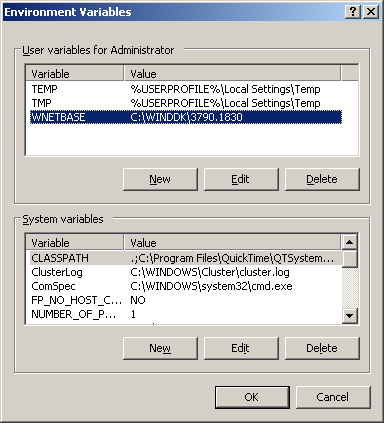
\includegraphics[width=0.6\textwidth]{./EnvironmentVars.png}
\end{figure}

\begin{figure}[h]
    \centering
    \caption{The Visual Studio 2005 \emph{Tools} dialog\label{fig:VisualStudioToolsDialog}}
    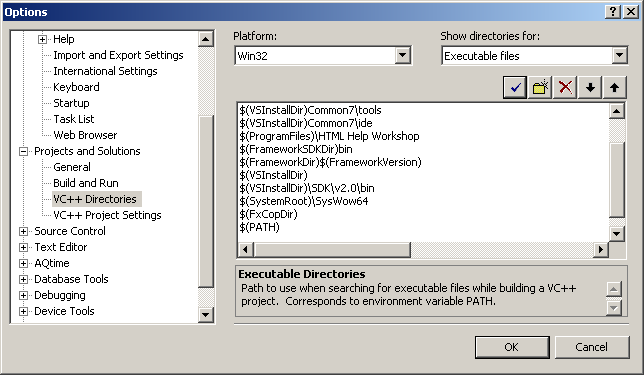
\includegraphics[width=\textwidth]{./VS2005_ExeDirs.png}
\end{figure}

\pagebreak\pdfbookmark[0]{Contents}{TOC}\tableofcontents\thispagestyle{fancy}
\end{document}
